\documentclass{beamer}

%\setbeamertemplate{background canvas}[vertical shading][top=blue!40]
%bottom=red!20,

% Escolhendo modo de apresentacao ideal
\mode<presentation>
{
  % http://www.pletscher.org/writings/latex/beamerthemes.php
  % http://www.hartwork.org/beamer-theme-matrix/
  % Possible themes:
  % Antibes, Bergen, Berkeley, Berlin, Boadilla, Copenhagen, Darmstadt,
  % Dresden, Frankfurt, Goettingen, Hannover, Ilmenau, JuanLesPins,
  % Luebeck, Madrid, Malmoe, Marburg, Montpellier, PaloAlto, Pittsburgh,
  % Rochester, Singapore, Szeged, Warsaw, boxes, default.

	% Com menu lateral
	%\usetheme{Berkeley}
	%\usetheme{Goettingen}
	%\usetheme{Hannover}
	\usetheme{Marburg}
	%\usetheme{PaloAlto}

	% Com menu superior
	%\usetheme{Montpellier}
	%\usetheme{Pittsburgh}
	
	% Sem Menu
	%\usetheme{Boadilla}
	%\usetheme{CambridgeUS}
	%\usetheme{Madrid}

	% Possible color themes: albatross beaver beetle crane default 
	%dolphin dove fly lily orchid rose seagull seahorse whale wolverine
	\usecolortheme{dolphin}
	
	%\setbeamercovered{transparent}

	%\usefonttheme[onlysmall]{structurebold}

	\setbeamertemplate{frametitle continuation}[from second][]
	\setbeamertemplate{navigation symbols}{} % retira a barra de navegação
	\setbeamertemplate{footline}[frame number] % coloca numero nas páginas
}

\usepackage[brazil]{polyglossia}
\usepackage{xltxtra}  % provides some fixes/extras

\usepackage{hyperref}
\hypersetup{%
	pdftitle={Criação de uma biblioteca padrão para HasCASL},%
	pdfauthor={Glauber M. Cabral},%
	pdfsubject={},%
	pdfkeywords={}%
}

%\setmonofont{Monaco}

\usepackage{relsize}
\usepackage{fancyvrb}
\fvset{fontsize=\relsize{-1}}
\usepackage{listings}
\usepackage{ifthen}

\usepackage{xspace}
\newcommand{\HasCASL}{\textsc{HasCasl}\xspace}
\newcommand{\CASL}{\textsc{Casl}\xspace}
\newcommand{\Hets}{\textsc{Hets}\xspace}
\newcommand{\Haskell}{\textsc{Haskell}\xspace}
\newcommand{\ML}{\textsc{ML}\xspace}
\newcommand{\HOL}{\textsc{HOL}\xspace}
\newcommand{\Isabelle}{\textsc{Isabelle}\xspace}
\newcommand{\Prelude}{\textsc{Prelude}\xspace}
\newcommand{\HOLCF}{\textsc{HOLCF}\xspace}
\newcommand{\SML}{\textsc{SML}\xspace}
\newcommand{\EML}{\textsc{EML}\xspace}
\newcommand{\Maude}{\textsc{Maude}\xspace}
\newcommand{\Larch}{\textsc{Larch}\xspace}
\newcommand{\Z}{\textsc{Z}\xspace}
\newcommand{\BMethod}{\textsc{Método B}\xspace}
\newcommand{\AMN}{\textsc{AMN}\xspace}

\title[Criação de uma Biblioteca Padrão para a Linguagem HasCASL]{Criação de uma Biblioteca Padrão para a Linguagem HasCASL}
\author[Glauber M. Cabral]{Glauber Módolo Cabral -- Orientando\\
Prof. Dr. Arnaldo Vieira Moura -- Orientador}
\institute[IC - UNICAMP]{
  \textbf{\large{Universidade Estadual de Campinas}}\par
  \textbf{\large{Instituto de Computação}}\par
\begin{figure}
	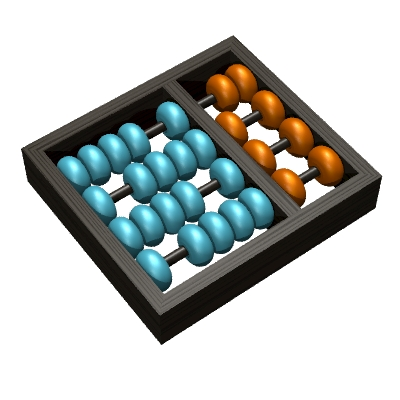
\includegraphics[scale=0.1]{figuras/Ic}
\end{figure}
}
\date{26 de Abril de 2010}
\subject{}
\logo{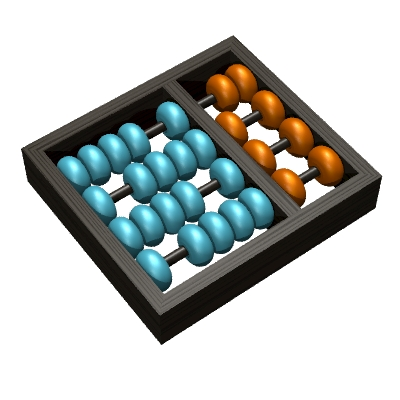
\includegraphics[scale=0.06]{figuras/Ic}}

\begin{document}

% ROTEIRO
% Introdução
% Linguagens relacionadas
% Linguagens utilizadas
% Motivação
% Objetivos
% Trabalho desenvolvido
% Contribuições
% Problemas encontrados e possíveis soluções
% Conclusões
% Trabalhos futuros
% Agradecimentos


%para criar a página de rosto
\frame{\titlepage} %inclui a front page

\section*{Roteiro}
% cria o sumário
\begin{frame}
  \frametitle{Roteiro}
  \tableofcontents
\end{frame}

\section{Introdução}

\subsection{Métodos Formais e Linguagens de Especificação}

\begin{frame}
	\frametitle{}
	\begin{block}{Métodos Formais}
		\begin{itemize}
			\item Ferramentas de Engenharia de Software que empregam formalismos matemáticos na construção de programas;
			\item Compostos por uma ou mais linguagens de especificação e algumas ferramentas auxiliares;
		\end{itemize}
	\end{block}

	\begin{block}{Linguagens de Especificação Formal}
		\begin{itemize}
			\item Linguagens existentes são baseadas em diversos formalismos: Extended ML, \Z, \BMethod, \Maude, \Larch, \CASL, \ldots);
			\item Apresentam variado nível de suporte à verificação automática de propriedades auxiliada por ferramentas.
			\item Possuem códigos de exemplo e bibliotecas para reuso.
		\end{itemize}
	\end{block}
\end{frame}

\section{Contextualização}

\subsection{Linguagens Utilizadas}

\begin{frame}	
\begin{block}{\CASL: Common Algebraic Specification Language}
	\begin{itemize}
		\item Linguagem de especificação algébrica que permite extensões e sub-linguagens;
		\item Possui uma biblioteca padrão com especificações para reuso.
	\end{itemize}
\end{block}

\begin{block}{\Haskell}
	\begin{itemize}
		\item Linguagem de programação funcional;
		\item Implementa conceitos de lógica de segunda ordem: tipos que são funções, polimorfismo e construtores de tipos;
		\item Avaliação preguiçosa: argumentos de função são avaliados apenas quando são usados;
		\item \Haskell \Prelude: biblioteca padrão com tipos básicos e funções de manipulação de listas, de textos e de E/S em tela e arquivo.
	\end{itemize}
\end{block}
\end{frame}

\begin{frame}

\begin{block}{\HasCASL: \Haskell + \CASL}
	\begin{itemize}
		\item Extensão de CASL com conceitos de lógica de segunda ordem;
		\item Tem a linguagem de programação funcional \Haskell como sub-conjunto;
			\begin{itemize}
				\item Facilita a transformação da especificação para código \Haskell executável;
			\end{itemize}
		\item Possui avaliação estrita: função com parâmetros indefinidos possui valor de retorno indefinido;
		\item No entanto, avaliação preguiçosa pode ser emulada por uma combinação de tipos de dados;
		\item \textbf{Não possui biblioteca padrão com especificações reutilizáveis.}
	\end{itemize}
\end{block}
\end{frame}

\subsection{Ferramentas Utilizadas}
\begin{frame}

\begin{block}{\Hets: Heterogeneous Tool Set}
	\begin{itemize}
		\item Analisador sintático para \CASL e sub-lingugens;
		\item Utiliza o editor \textit{Emacs} como interface.
		\item Gera um \textit{Grafo de Desenvolvimento}:
			\begin{itemize}
				\item Nós: especificações;
				\item Arcos: dependência entre especificações;
				\item Cores indicam o estado das necessidades de prova;
			\end{itemize}
		\item Gerencia as provas realizadas com o provador de teoremas \Isabelle.
	\end{itemize}
\end{block}

\begin{block}{Isabelle}
	\begin{itemize}
		\item Provador de teoremas semi-automático;
		\item Lógicas para escrita de provas: \HOL e \HOLCF, dentre outras;
		\item \Hets traduz especificações em \HasCASL para \HOL  e \HOLCF.
	\end{itemize}
\end{block}
\end{frame}

\begin{frame}
\begin{figure}
\centering
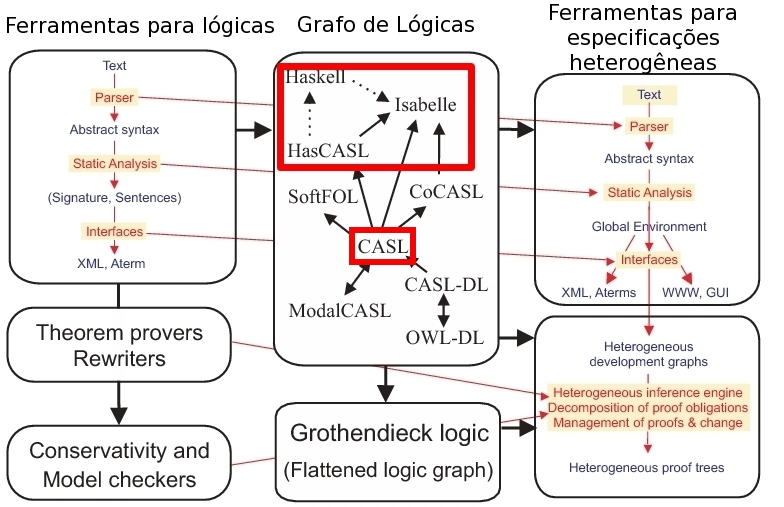
\includegraphics[height=0.72\textheight]{figuras/hets-new}
\end{figure}
{\tiny{Fonte:\\ http://www.informatik.uni-bremen.de/agbkb/\allowbreak{}forschung/\allowbreak{}formal\_methods/\allowbreak{}CoFI/hets/index\_e.htm}}
\end{frame}

\section{Motivação e Justificativa}

\begin{frame}
	\frametitle{Motivação e Justificativa}
	\begin{block}{Criação de uma Biblioteca Padrão para \HasCASL}
	\begin{itemize}
		\item Contribuiria para difundir a linguagem;
		\item Permitiria o reuso de especificações;
		\item Considerada uma premissa para uso da linguagem em problemas reais.
	\end{itemize}
	\end{block}
	\begin{block}{Biblioteca \Prelude como Ponto de Partida}
	\begin{itemize}
		\item Possui tipos de dados amplamente utilizados em programas Haskell;
		\item Permitiria o uso de tipos existentes em \Haskell nas especificações escritas em \HasCASL;
		\item Facilitaria a transformação de especificações em \HasCASL para código executável em \Haskell;
	\end{itemize}
	\end{block}
\end{frame}

\section{Objetivos}

\begin{frame}
	\frametitle{Objetivos}
	\begin{block}{Objetivo Principal}
		Especificar uma biblioteca para a linguagem \HasCASL com tipos de dados de segunda ordem segundo a biblioteca \Prelude da linguagem \Haskell.
	\end{block}
	\begin{block}{Objetivo Secundário}
		Provar teoremas criados pela ferramenta Hets durante a análise da especificação utilizando o provador de teoremas \Isabelle.
	\end{block}
\end{frame}

\section{Desenvolvimento}

\begin{frame}
	\frametitle{Escolhas iniciais}
	
	\begin{block}{Avaliação Estrita}
	\begin{itemize}
		\item Emprega construções mais simples de \HasCASL;
		\item Precisa de conhecimento básico de \HOL para escrever as provas;
		\item Possui alguma documentação e alguns exemplos;
		\item Escolhida como ponto de partida para a especificação.
	\end{itemize}
	\end{block}
	
	\begin{block}{Avaliação Preguiçosa}
	\begin{itemize}
		\item Emprega construções mais avançadas de \HasCASL;
		\item Precisa de profundo conhecimento prévio das linguagens \HOL e \HOLCF para escrever as provas;
		\item Possui pouca documentação e exemplos;
		\item Introduzida em refinamento posterior da especificação.
	\end{itemize}
	\end{block}
\end{frame}

\begin{frame}
	\begin{block}{Especificação da Biblioteca em \HasCASL}
	\begin{itemize}
		\item Modela tipos e funções através de axiomas em \HasCASL e \CASL;
		\item Possui propriedades a serem verificadas com \Isabelle.
		\item Constituída por 18 especificações.
	\end{itemize}
	\end{block}
\end{frame}

\begin{frame}
	\begin{block}{Verificação de Teoremas com \Isabelle}
	\begin{itemize}
		\item Garante que as especificações se comportem como eperado;
		\item Necessita que axiomas sejam reescritos para que \Isabelle consiga usá-los;
		\item Axiomas são reescritos na forma de lemas e também precisam ser provados para garantir consistência;
	\end{itemize}
	\end{block}
\end{frame}

\begin{frame}
	\frametitle{Estado Inicial da Verificação das Especificações}
\begin{figure}
\centering
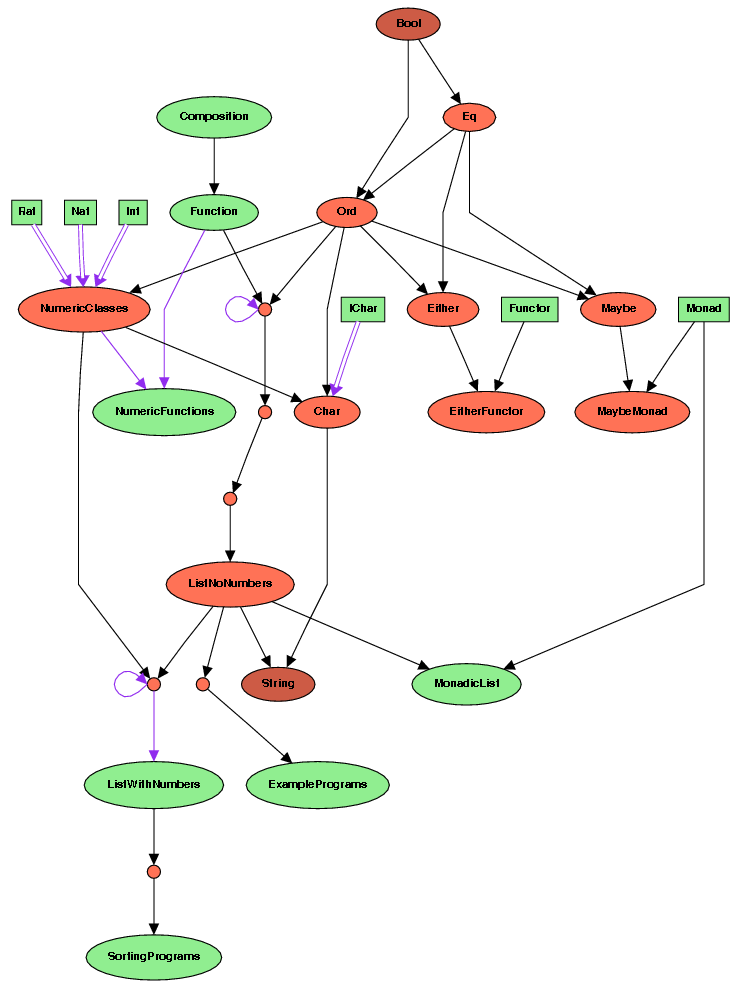
\includegraphics[height=0.9\textheight]{figuras/ProofStart.png}
\end{figure}
\end{frame}

\begin{frame}[containsverbatim]
	\frametitle{Especificação Ord em \HasCASL}

\renewcommand{\FancyVerbFormatLine}[1]{% 
	\ifthenelse{%
		\equal{\value{FancyVerbLine}}{10}%
		\or%
		\equal{\value{FancyVerbLine}}{11}%
		\or%
		\equal{\value{FancyVerbLine}}{12}%
		\or%
		\equal{\value{FancyVerbLine}}{13}%
	}{%
	 	\textcolor{red!60!black}{#1}%
	}{%
		{#1}%
	}%
}
	
\begin{Verbatim}[numbers=left,numbersep=3pt]
spec Ord = Eq and Bool then
free type Ordering ::= LT | EQ | GT
type instance Ordering: Eq
 . (LT == LT) = True   %(IOE01)% %implied
 . (LT == EQ) = False  %(IOE04)%
 . (LT /= EQ) = True   %(IOE07)% %implied
class Ord < Eq {
 fun __<__ : a * a -> Bool
 var x, y, z, w: a
 . (x == y) = True => (x < y) = False
                                  %(LeIrreflexivity)%
 . (x < y) = True => y < x = False
                            %(LeTAsymmetry)% %implied
 . (x < y) = True /\ (y < z) = True
  => (x < z) = True                 %(LeTTransitive)%
 . (x < y) = True \/ (y < x) = True
  \/ (x == y) = True                     %(LeTTotal)%
}
\end{Verbatim}
\end{frame}

\begin{frame}[containsverbatim]
	\frametitle{Especificação Ord traduzida para \HOL}
	
\renewcommand{\FancyVerbFormatLine}[1]{% 
	\ifthenelse{%
		\value{FancyVerbLine}<6%
		\or%
		\value{FancyVerbLine}>7%
		\and%
		\value{FancyVerbLine}<11%
	}{%
	 	\textcolor{red!60!black}{#1}%
	}{%
		\ifthenelse{%
			\value{FancyVerbLine}=6%
			\or%
			\value{FancyVerbLine}>10%
			\and%
			\value{FancyVerbLine}<17%
		}{%
		 	\textcolor{green!60!black}{#1}%
		}{%
			{#1}%
		}%
	}%
}

\begin{Verbatim}[numbers=left,numbersep=3pt]
LeIrreflexivity [rule_format] :
"ALL (x :: 'a). ALL (y :: 'a).
 x ==' y = True' --> x <' y = False'"

lemma LeIrreflContra : " x <' x = True' ==> False"
by auto

theorem LeTAsymmetry :
"ALL (x :: 'a). ALL (y :: 'a).
 x <' y = True' --> y <' x = False'"
apply(auto)
apply(rule ccontr)
apply(simp add: notNot2 NotTrue1)
apply(rule_tac x="x" in LeIrreflContra)
apply(rule_tac y = "y" in LeTTransitive)
by auto
\end{Verbatim}
\end{frame}

\begin{frame}[allowframebreaks]{Passo a passo da Especificação e Verificação}

	\begin{enumerate}
		\item Realizar verificação sintática com a ferramenta \Hets no arquivo da especificação (extensão \textit{.casl} ou \textit{.het});
		\begin{figure}
			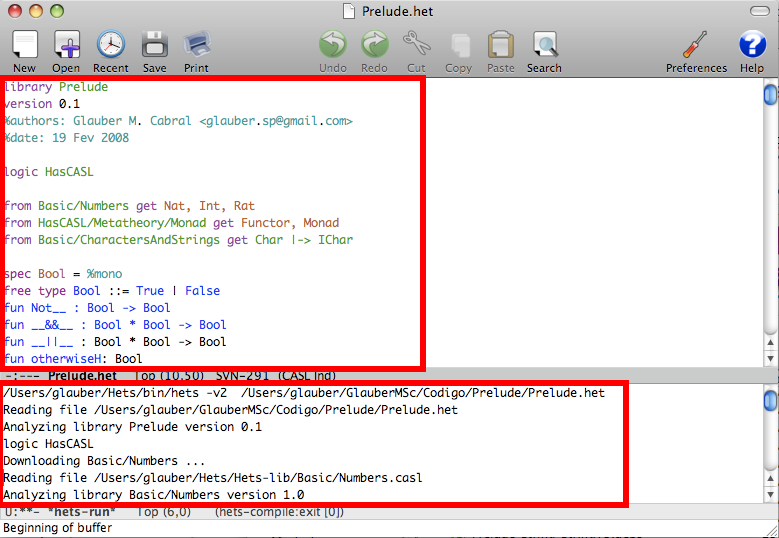
\includegraphics[height=0.68\textheight]{figuras/passo_a_passo/Picture01.png}
		\end{figure}
		
		\item \Hets gera o grafo de desenvolvimento da especificação analisada;
		\begin{figure}
			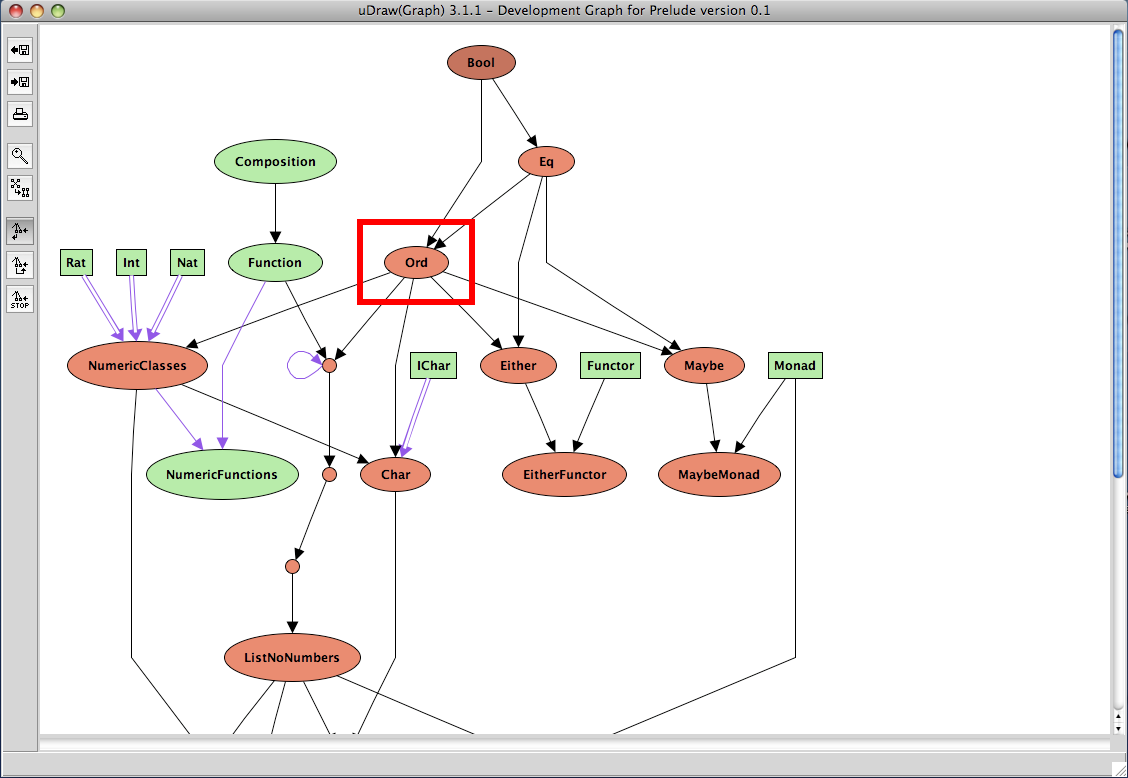
\includegraphics[height=0.7\textheight]{figuras/passo_a_passo/Picture02.png}
		\end{figure}
		
		\item Executar o comando de prova automático para que ele interprete o grafo e as necessidades de prova;
		\begin{figure}
			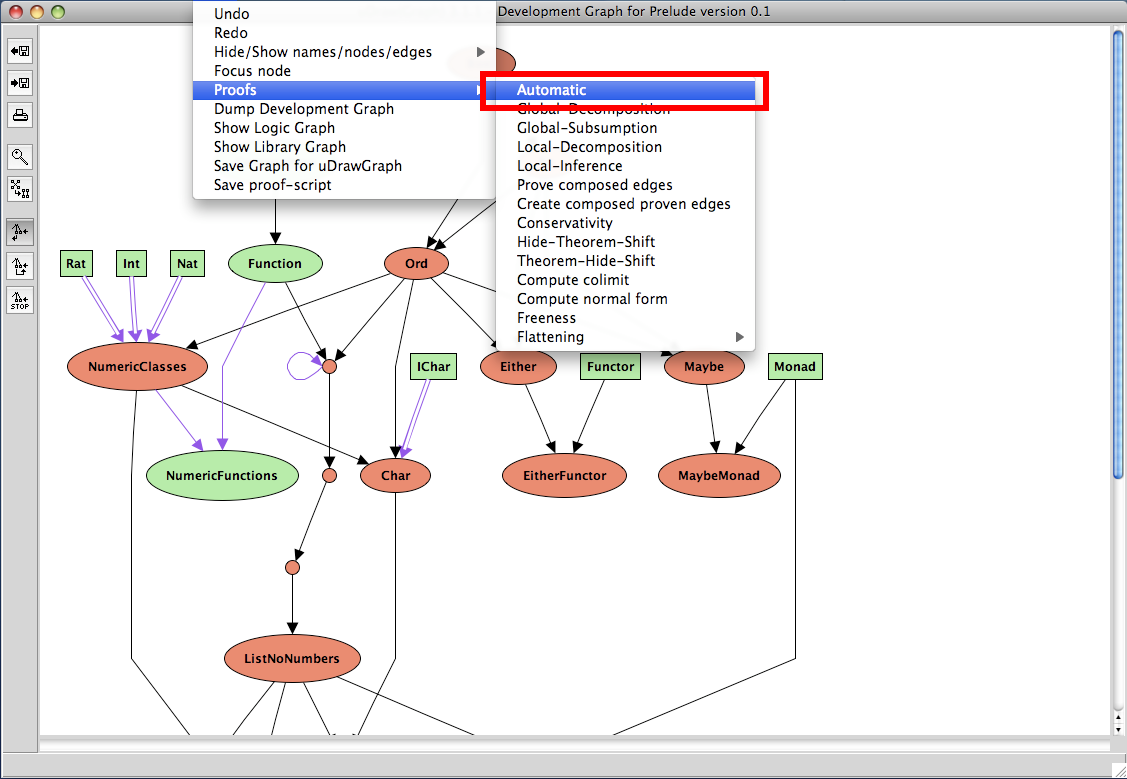
\includegraphics[height=0.7\textheight]{figuras/passo_a_passo/Picture03.png}
		\end{figure}
		
		\item Selecionar um nó vermelho (com provas em aberto) para verificar seus teoremas;
		\begin{figure}
			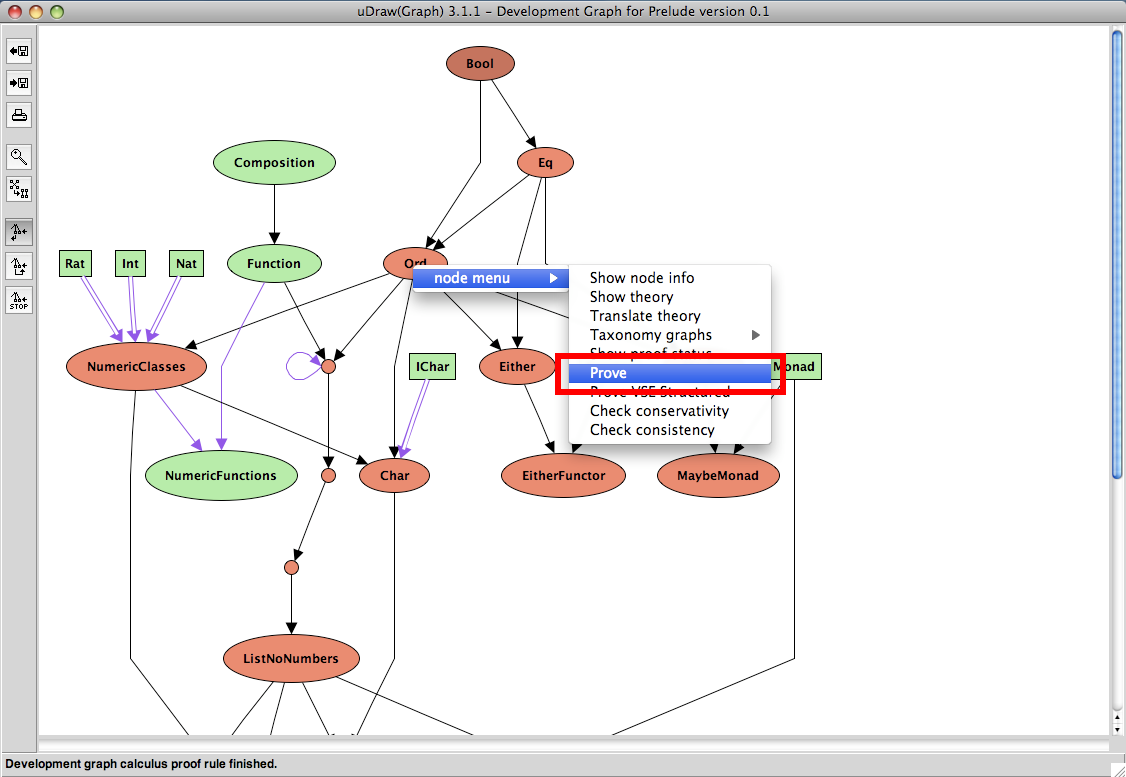
\includegraphics[height=0.7\textheight]{figuras/passo_a_passo/Picture04.png}
		\end{figure}
		
		\item Escolher os teoremas a serem provados, o provador de teorema e iniciar a prova;
		\begin{figure}
			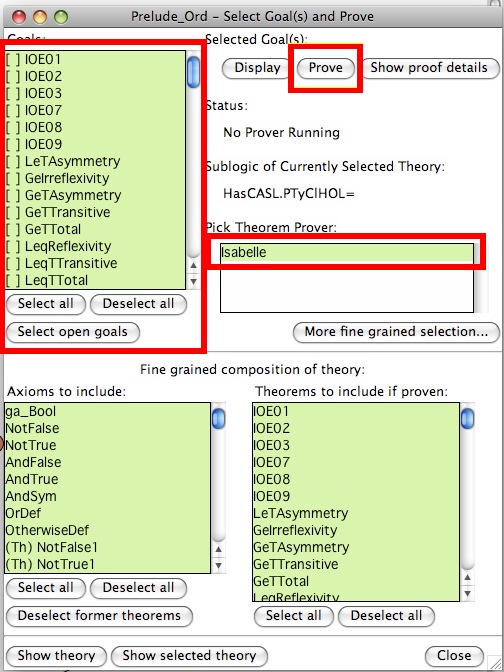
\includegraphics[height=0.7\textheight]{figuras/passo_a_passo/Picture05.png}
		\end{figure}
		
		\item Escrever as provas utilizando a interface \textit{ProofGeneral} para o provador \Isabelle;
		\begin{figure}
			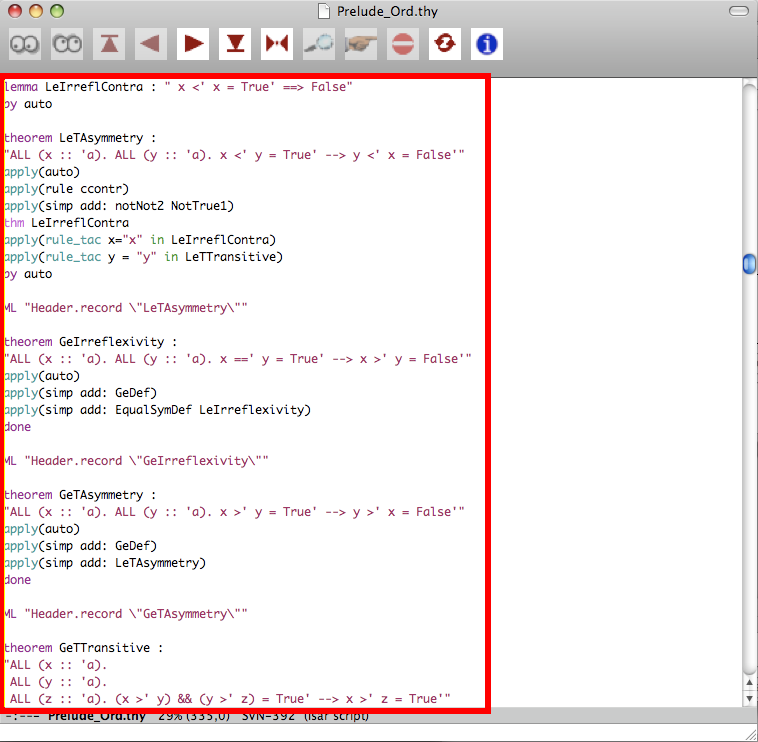
\includegraphics[height=0.7\textheight]{figuras/passo_a_passo/Picture06.png}
		\end{figure}

		\framebreak
		\item Executar a verificação completa do arquivo de prova e fechar a janela;
		\begin{figure}		
			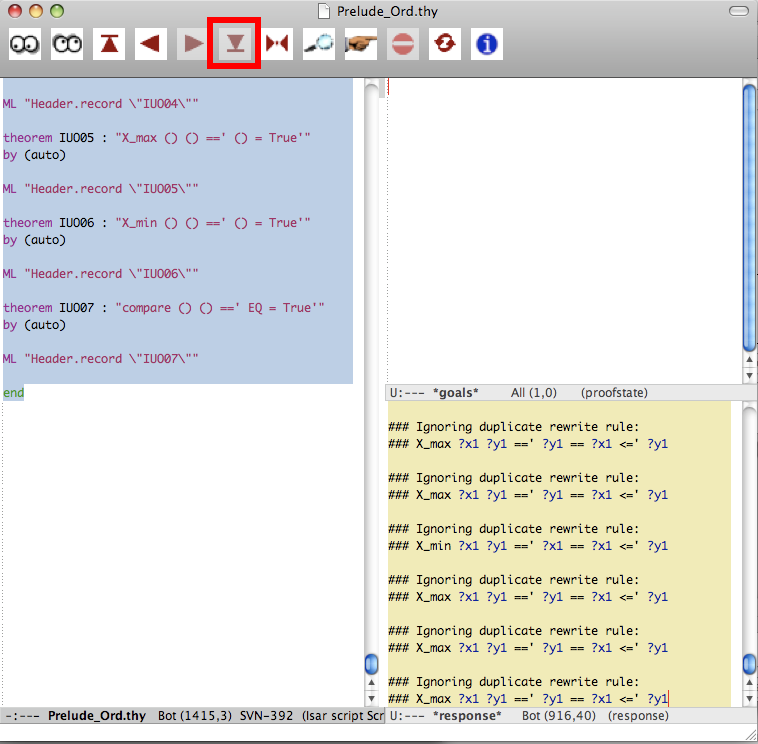
\includegraphics[height=0.7\textheight]{figuras/passo_a_passo/Picture07.png}
		\end{figure}
		
		\item Os teoremas que foram provados tem as respectivas caixas de seleção marcadas;
		\begin{figure}
			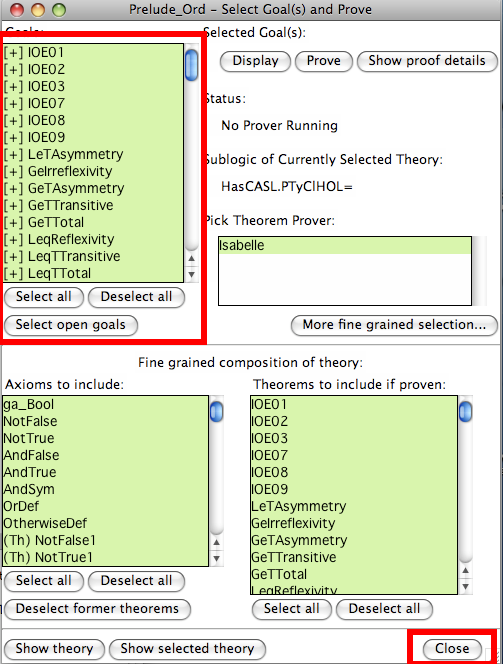
\includegraphics[height=0.7\textheight]{figuras/passo_a_passo/Picture08.png}
		\end{figure}
		
		\item Resultado da verificação no grafo: verde (totalmente verificado), vermelho (teoremas em aberto), amarelo (falta verificação de consistência).
	\end{enumerate}
	\begin{figure}
		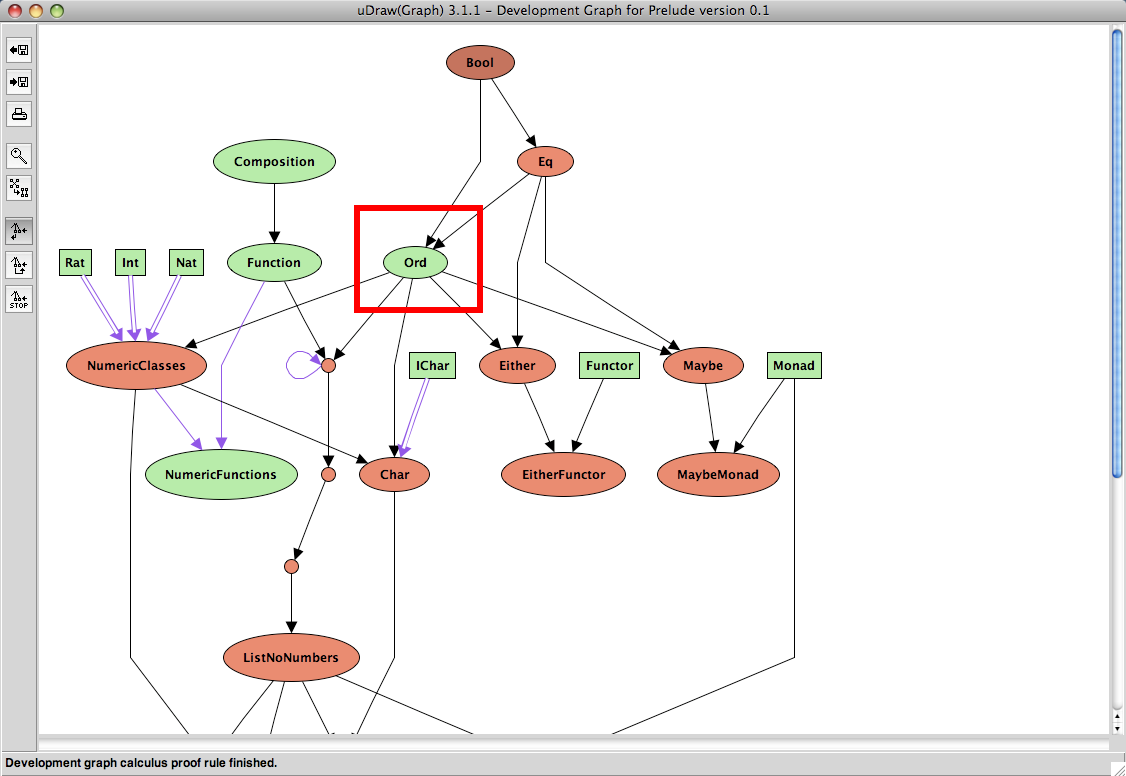
\includegraphics[height=0.64\textheight]{figuras/passo_a_passo/Picture09.png}
	\end{figure}

\end{frame}

\begin{frame}
	\frametitle{Estado Final da Verificação das Especificações}
\begin{figure}
\centering
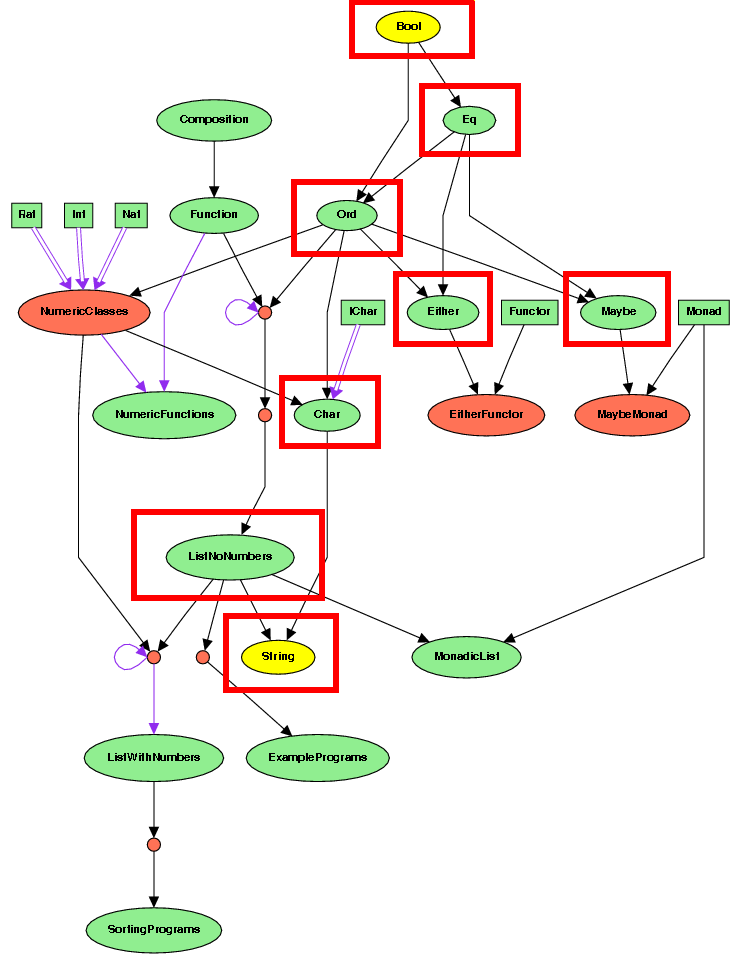
\includegraphics[height=0.9\textheight]{figuras/ProofEnd.png}
\end{figure}
\end{frame}

\section{Contribuições}

\begin{frame}
	\frametitle{Contribuições}
	
	\begin{itemize}
		\item Biblioteca especificada possui os tipos de dados booleano, listas, caracteres e cadeias de caracteres.
		\item Especificações de exemplos empregam listas e booleanos;
		\item Duas versões para a biblioteca (aprox. 1000 LOC cada):
		\begin{description}
			\item[$1^{a}$ Versão] Tipos com avaliação estrita devido à complexidade do uso de tipos com avaliação preguiçosa;
			\item[$2^{a}$ Versão] Refinamento para suportar tipos com avaliação preguiçosa sem suporte a tipos infinitos;
		\end{description}
		\item A maioria das necessidades de prova foram verificadas:
			\begin{itemize}
		 		\item 9 especificações verificadas totalmente;
				\item 8 especificações possuem alguns teoremas em aberto.
			\end{itemize}
	\end{itemize}
\end{frame}

\section{Questões em aberto}

\begin{frame}
	\frametitle{Questões em aberto}
	
	\begin{block}{Especificações de Tipos Numéricos}
	\begin{itemize}	
		\item Especificações de tipos numéricos da biblioteca da linguagem \CASL não possuem todos os lemas necessários para que sejam utilizadas com o provador \Isabelle.
		\item Seu uso exigiria mapeamentos entre os tipos de dados da biblioteca da linguagem \CASL e seus respetivos tipos de dados na linguagem \HOL.
		\item O mapeamento para o tipo de dados \texttt{Nat} hoje existente está implementado com funções obsoletas e não pode ser usado dentro do provador \Isabelle.
		\item Funções envolvendo tipos numéricos não foram especificadas na versão atual da biblioteca.
	\end{itemize}
	\end{block}
\end{frame}

\begin{frame}
	\frametitle{Questões em aberto}

	\begin{block}{Tipos Contínuos e Estruturas Infinitas}
	\begin{itemize}
		\item Exige tipos de dados complexos da linguagem \HasCASL e o uso da lógica \HOLCF no provador de teoremas \Isabelle.
		\item \HOLCF é mais complexa do que \HOL e seu uso estava fora do escopo do trabalho.
		\item Suporte a estes tipos não foi implementado;
		\item Por consequência, ainda não é possível refinar as especificações para o subconjunto executável da linguagem \HasCASL.
	\end{itemize}
	\end{block}
\end{frame}

\section{Conclusões}
\begin{frame}
	\frametitle{Conclusões}
	
	\begin{block}{Objetivos Iniciais}
	\begin{itemize}
		\item Especificar uma biblioteca para \HasCASL baseada na biblioteca \Prelude;
		\item Verificar propriedades das especificações criadas.
	\end{itemize}
	\end{block}
	
	\begin{block}{Objetivos Alcançados}
	\begin{itemize}
		\item Biblioteca possui os tipos de dados booleano, listas, caracteres e cadeias de caracteres
		\item Tipos numéricos, Tipos Contínuos e Estruturas Infinitas não foram especificados;
		\item Estado das necessidades de prova geradas:
			\begin{itemize}
				\item 9 totalmente verificadas;
				\item 8 verificadas parcialmente.
			\end{itemize}
	\end{itemize}
	\end{block}
\end{frame}

\section{Trabalhos futuros}

\begin{frame}
	\frametitle{Trabalhos Futuros}
	
	\begin{itemize}
		\item Escrever novos mapeamentos entre os tipos de dados da biblioteca da linguagem \CASL e os tipos de dados da linguagem \HOL
		\item Especificar e verificar tipos de dados numéricos e funções que os envolvam.
		\item Especificar tipos de dados infinitos;
		\item Expecificar estruturas de dados mais complexas implementadas por alguns compiladores da linguagem \Haskell.
	\end{itemize}
\end{frame}

\section{Agradecimentos}

\begin{frame}
  \frametitle{Agradecimentos}

\begin{block}{Obrigado!}
\end{block}

\begin{block}{Apoio Financeiro}
	\begin{figure}
	      
\includegraphics[scale=0.3]{figuras/cnpq}
	  \end{figure}
\end{block}

\begin{block}{Contato}
glauber.sp@gmail.com
\end{block}
\end{frame}



\end{document}